% !TEX root = ../main.tex
%-------------------------------------------------------------------------------
%-------------------------------------------------------------------------------
\begin{frame} I draw on the material presented in:\vspace{0.3cm}

\begin{itemize}\setlength\itemsep{1em}
  \item \bibentry{Gorelick.2014}
  \item \bibentry{Lanaro.2017}
\end{itemize}
\end{frame}
%-------------------------------------------------------------------------------
%-------------------------------------------------------------------------------
\begin{frame}\textbf{Basic architecture}\vspace{0.3cm}

\begin{itemize}\setlength\itemsep{1em}
    \item computing units, e.g. CPU and GPU
    \item memory units, e.g. RAM and hard disk
    \item connections
\end{itemize}

\end{frame}
%-------------------------------------------------------------------------------
%-------------------------------------------------------------------------------
\begin{frame}\textbf{Main properties of computing unit}\vspace{0.3cm}

\begin{itemize}\setlength\itemsep{1em}
    \item number of operations in one cycle, e.g. vectorization
    \item how many cycles in one second
\end{itemize}

\end{frame}
%-------------------------------------------------------------------------------
%-------------------------------------------------------------------------------
\begin{frame}\textbf{Global interpreter lock}\vspace{0.3cm}

\begin{quote} The GIL makes sure that a Python process can only run one instruction at a time, regardless of the number of cores it is currently using. This means that even though some Python code has access to multiple cores at a time, only one core is running a Python instruction at any given time.
\end{quote}
\end{frame}
%-------------------------------------------------------------------------------
%-------------------------------------------------------------------------------
\begin{frame}\textbf{Profiling}\vspace{0.3cm}

\begin{itemize}\setlength\itemsep{1em}
    \item \textit{Premature optimization is the root of all evil.}
    \item focus on readability
    \item set up development environment
    \item flesh out testing harness
    \item tackle performance bottlenecks
\end{itemize}

\end{frame}
%-------------------------------------------------------------------------------
%-------------------------------------------------------------------------------
\begin{frame}\textbf{Points of attack}\vspace{0.3cm}

\begin{itemize}\setlength\itemsep{1em}
    \item pure Python
    \item high-performance libraries, SciPy Stack
    \item compilation to faster language
    \item parallel computing
    \item distributed computing
\end{itemize}

\end{frame}
%-------------------------------------------------------------------------------
%-------------------------------------------------------------------------------
\begin{frame}
	\begin{figure}[htp]\centering
    \scalebox{0.3}{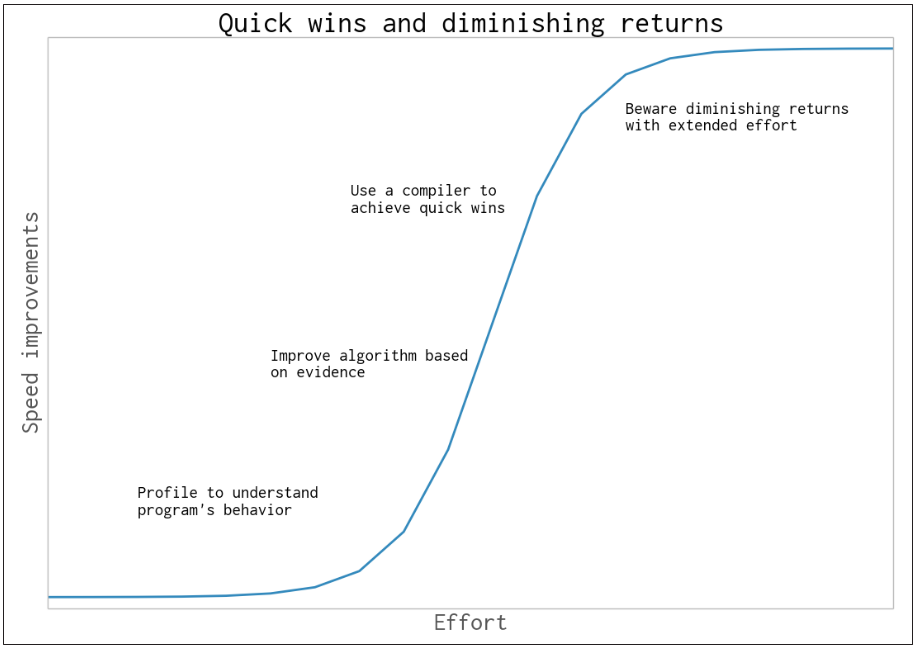
\includegraphics{fig-diminishing-returns}}
	\end{figure}
\end{frame}
